\documentclass{IEEEtran}
%% PACKAGES %%

\usepackage{amsmath, amsfonts, amssymb, amsthm}
\usepackage{braket}
\usepackage{listings}
\usepackage{geometry}
\usepackage{xcolor}
\usepackage{textcomp}
\usepackage{graphicx}
\usepackage{fancyhdr}
\usepackage{sourcecodepro}
\usepackage{multirow}

%%%%%%%%%%%%%%

\graphicspath{{./images}}
\setlength\parindent{0pt}       % globally supress indentation

%% LISTINGS CONFIG %%

\definecolor{purple2}{RGB}{153,0,153} % there's actually no standard purple
\definecolor{green2}{RGB}{0,153,0} % a darker green

\lstset{
  language=MATLAB,                   % the language
  basicstyle=\normalsize\ttfamily,   % size of the fonts for the code
  frame = single,
  % Color settings to match IDLE style
  keywordstyle=\color{orange},       % core keywords
  keywordstyle={[2]\color{purple2}}, % built-ins
  stringstyle=\color{green2},%
  showstringspaces=false,
  commentstyle=\color{red},%
  upquote=true,                      % requires textcomp
  numbers=left,
  breaklines=true,
}

% Title Stuff
\title{\vspace{-3cm} Filter Design}
\author{Chase A. Lotito, \textit{SIUC Undergraduate}}
\date{}

\begin{document}

\pagestyle{fancy}

% attempt to make nice header
\fancyhead{}
\fancyhead[CH]{\normalsize{LOTITO - SIUC - ECE355L Project 5}}

\maketitle % Makes the title

\section{Experimental Results}

\subsection{Task I: FIR Filter}

\begin{figure}[!ht] 
    \centering
    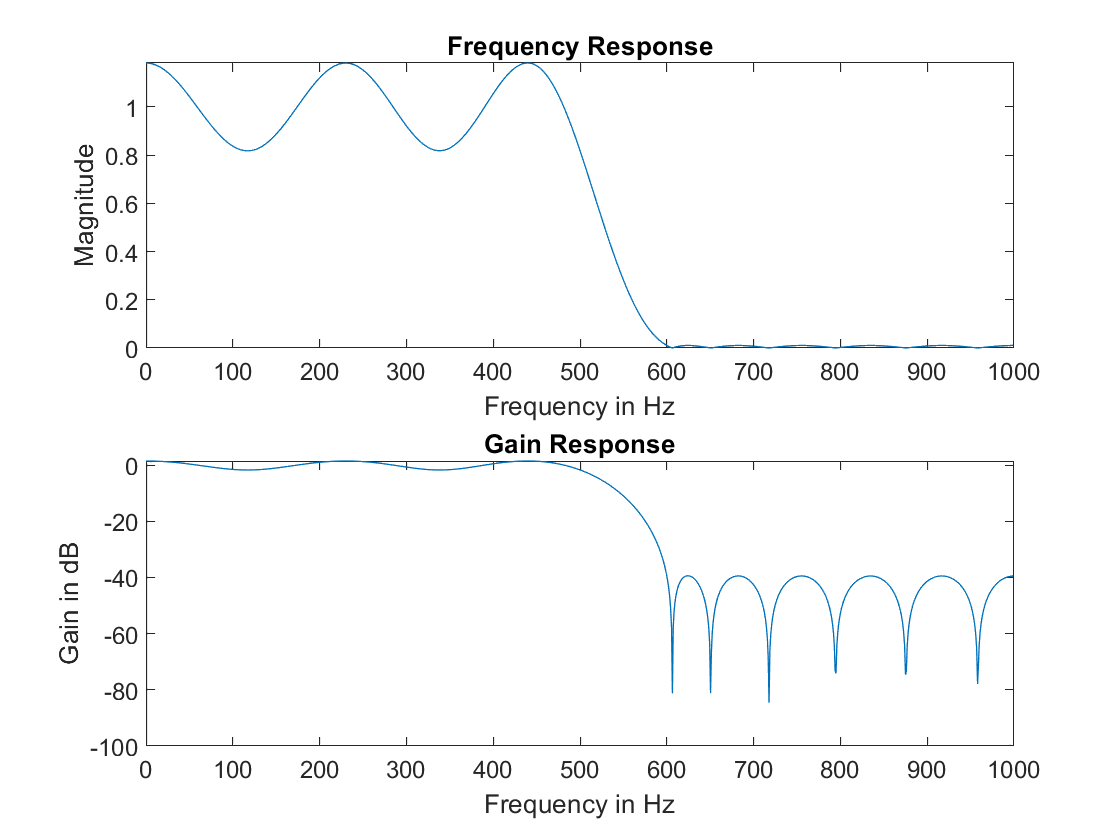
\includegraphics[width = 7cm]{task1.png}
    \caption{FIR low-pass filter.}
    \label{fig:task1}
\end{figure}

\subsection{Task II: Butterworth and Chebyshev IIR Filters}

\begin{figure}[!ht] 
    \centering
    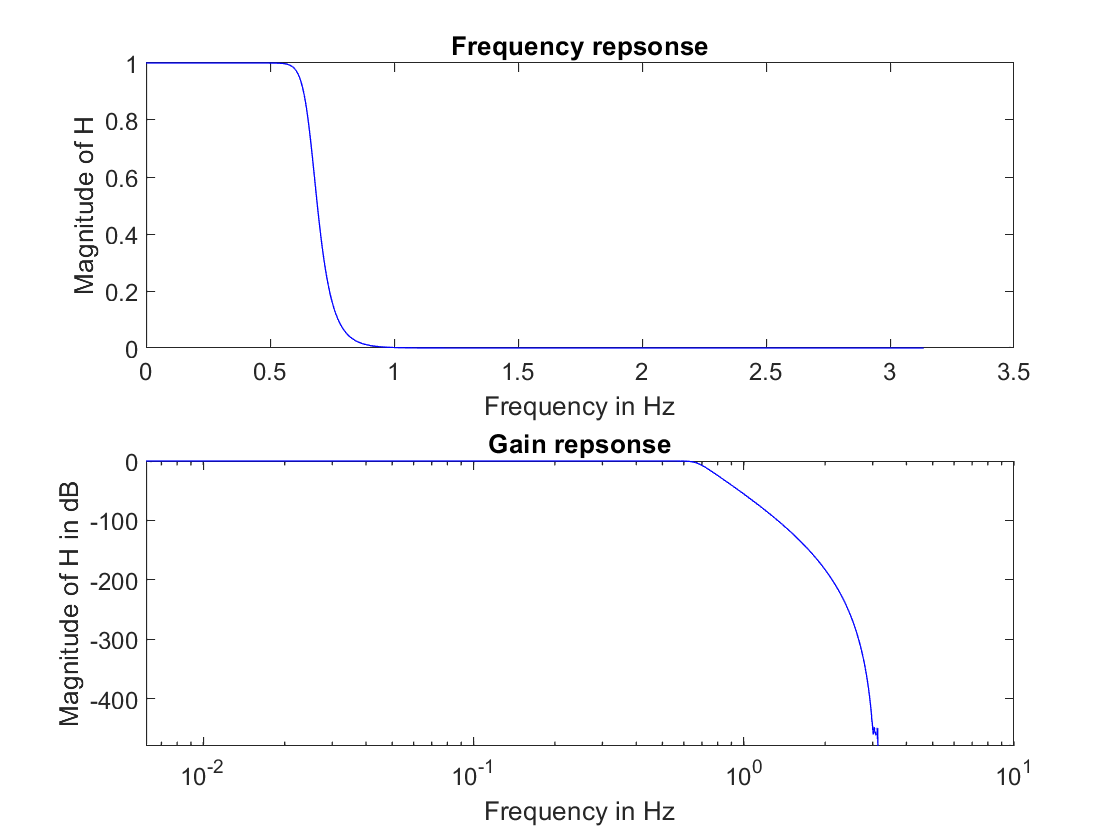
\includegraphics[width = 7cm]{butterworth.png}
    \caption{IIR Butterworth filter.}
    \label{fig:butterworth}
\end{figure}

\begin{figure}[!ht] 
    \centering
    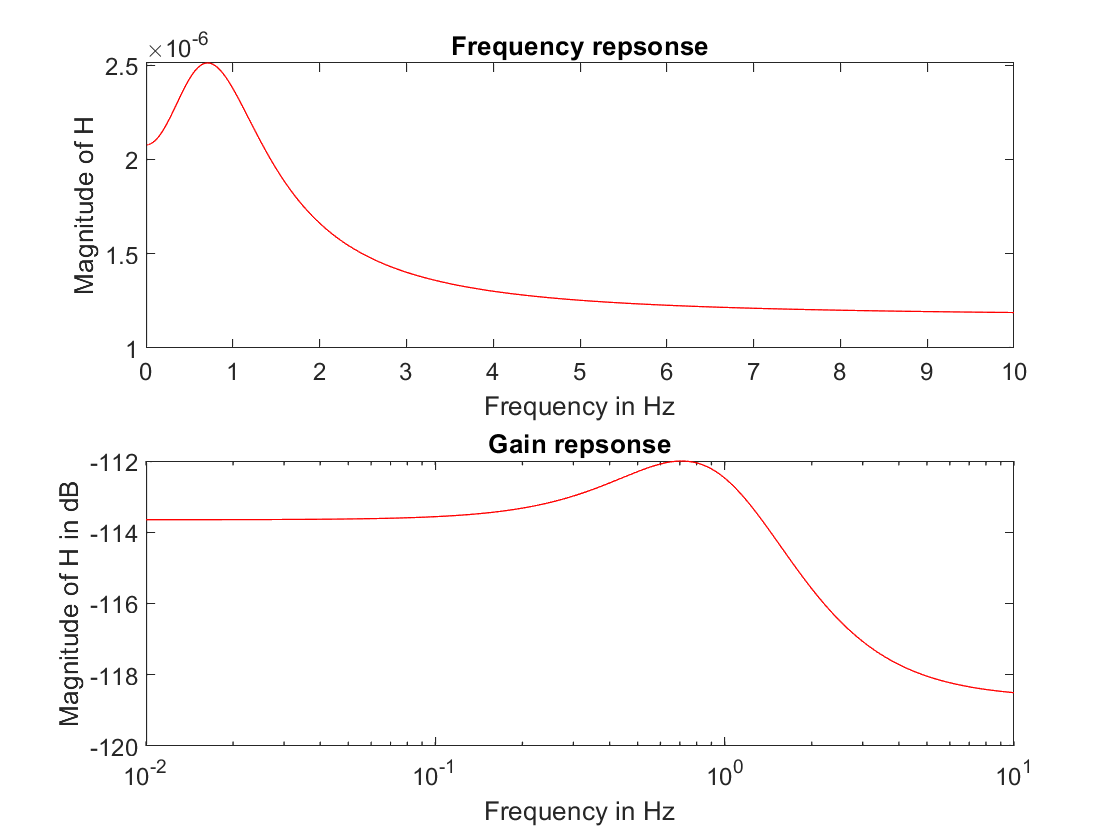
\includegraphics[width = 7cm]{chebyshev.png}
    \caption{IIR Chebyshev filter.}
    \label{fig:chebyshev}
\end{figure}

\section{Discussion}
% Please discuss your understanding of the digital filter design with considerations of public health, safety, and welfare, as well as global, cultural, social, environmental, and economic factors. (This discussion could be in general and should not be limited to the tasks of IIR and FIR filters design).

% TODO: put references
\bibliographystyle{IEEEtran}
\bibliography{project5Bib.bib}

\end{document}
